\chapter{Messungen}
\label{cha:Messungen}
    Im Rahmen dieser Arbeit wurden verschiedene Messungen und Benchmarks des Laufzeitverhaltens durchgeführt, um Vergleiche zwischen den bereits bekannten Technologien und den Neuerungen in Projekt Loom 
    durchführen zu können. 

\section{Testumgebung}                                         
\label{sec:Testumgebung}

    Alle getesteten Programme wurden mittels Java Development Kit (JDK) \emph{Eclipse Temurin 22.0.2} kompiliert und ausgeführt. Als JVM-Optionen wurden 
\begin{verbatim}
--add-exports java.management/sun.management=ALL-UNNAMED 
--add-exports jdk.management/com.sun.management.internal=ALL-UNNAMED 
-XX:+UnlockDiagnosticVMOptions -XX:+DebugNonSafepoints\end{verbatim}
    benutzt.
    Das System nutzt Windows 10 Professional als Betriebssystem und ist mit einem "i7-8086K" Prozessor ausgestattet. Dabei handelt es sich um eine CPU mit x86-64-Anweisungssatz und 6 
    Kernen mit einer Taktfrequenz zwischen 4 und 5 GHz. Als Arbeitsspeicher kamen  16 GB DDR4-RAM zum Einsatz, welche auf 2600MHz takten. Die integrierte Graphikeinheit der CPU wurde, 
    um eine zusätzliche Wärmebelastung zu vermeiden, deaktiviert. 
    Für die Laufzeitmessungen wurde das "Java Microbenchmark Harness (JMH)" Version 1.37 verwendet.
    Es wurden keine Maßnahmen ergriffen, um hardwarespezifische Einflussfaktoren wie den Taktraten-Boost der CPU zu unterbinden.


\section{Laufzeitmessungen bei Threads in verschiedenen Szenarien}                                         
\label{sec:LaufzeitmessungenbeiThreadsinverschiedenenSzenarien}

    Um die Stärken und Schwächen von \Glspl{vt} im Vergleich zu \Glspl{pt} genauer ermitteln bzw. evaluieren zu können, sind Laufzeitmessungen in verschiedenen Szenarien nötig. 
    Anhand dieser Messungen kann ein Leitfaden für die Wahl zwischen \Glspl{pt} und \Glspl{vt} erstellt werden. 
    Folgende Szenarien werden behandelt:
    \begin{itemize}
        \item Laufzeitmessungen unter hoher Auslastung (CPU-intensive Berechnungen),  
        \item Laufzeitmessungen bei sehr vielen Threads und blockierenden (wartenden) Aufgaben.
        \item Laufzeitmessungen bei einer Abhängigkeit zwischen Threads und Verwendung einer geteilten Ressource.
    \end{itemize}


\subsection{Laufzeitmessungen bei Threads unter hoher CPU-Auslastung}                                         
\label{subsec:LaufzeitmessungenbeiThreadsunterhoherAuslastung}

    Ziel der ersten Laufzeitmessung war es herauszufinden wie sich \Glspl{vt} unter ständiger hoher Auslastung schlagen. Die vom Thread ausgeführte Aufgabe greift auf keine 
    externen Ressourcen zu und weist auch keine Abhängigkeiten von anderen Prozessen auf. Die Berechnungen sind daher ohne Unterbrechung durchführbar.
    Dieser Vergleich nutzt dadurch keine der von den Entwicklern erwähnten  Stärken von \Glspl{vt}.
    \begin{program} [H]
        \caption{Benchmark eines \Glspl{vt} unter hoher Auslastung}
        \label{prog:BenchmarkEinesVTUnterHoherAuslastung}
    \begin{JavaCode}[language=Java, numbers=left]
@State(Scope.Benchmark)
public class PerformanceVirtual {

    @Param("10000")
    public int nonsenseIterations;

    @Benchmark
    @BenchmarkMode(Mode.SampleTime)
    @OutputTimeUnit(TimeUnit.MILLISECONDS)
    public void testMethodeVirtual() throws InterruptedException {
        Thread.startVirtualThread(() -> {
            for (int i = 0; i < nonsenseIterations; i++)
                Utility.executeNonsense();
        }).join();
    }
}\end{JavaCode}
    \end{program}
    Dieser Benchmark startet einen \gls{vt} und lässt ihn durchgängige rechenintensive Aufgaben erledigen. Um eine Messung durchführen zu können, wartet der Eltern-Thread auf
    die Beendung der Aufgaben. Um den Unterschied in der Laufzeit sichtbarer zu gestalten und die Auswirkungen externer Störungsfaktoren zu minimieren,
    wird die Berechnung wiederholt ausgeführt. Die Anzahl der Ausführungen ist in Zeile 4 definiert. Der Methodenaufruf \texttt{executeNonsense()} in Zeile 13 stellt die Berechnung dar.
    Die Methode wird in \ref{prog:executeNonsense} näher erklärt. Der Benchmark für die \gls{pt} ist bis auf die Art des verwendeten Threads ident.
    Als Ergebnis wird die gesamte Dauer der Ausführung geliefert. 

    \begin{program} [H]
        \caption{Rechenintensive Prozedur}
        \label{prog:executeNonsense}
    \begin{JavaCode}[language=Java, numbers=left]
public static void executeNonsense() {
    int limit = 100000; // Adjust this limit for more or less intensity
    boolean[] isPrime = new boolean[limit + 1];
    for (int i = 2; i <= limit; i++) 
        isPrime[i] = true;
    for (int factor = 2; factor * factor <= limit; factor++) {
        if (isPrime[factor]) {
            for (int j = factor; factor * j <= limit; j++) 
                isPrime[factor * j] = false;
        }
    }
    int primeCount = 0;
    for (int i = 2; i <= limit; i++) {
        if (isPrime[i])
            primeCount++;
    }
}\end{JavaCode}
    \end{program}

    Die Methode \texttt{executeNonsense} in \ref{prog:executeNonsense} errechnet alle Primzahlen zwischen 2 und einer in Zeile 2 definierten Obergrenze. Anschließend wird 
    auch noch die Anzahl der Primzahlen ermittelt. Das Ergebnis ist komplett irrelevant und wird nach der Berechnung nicht weiterverwendet. Wichtig ist nur, dass es sich um
    eine aufwändige Berechnung handelt.

    \begin{figure}[H]
        \centering
        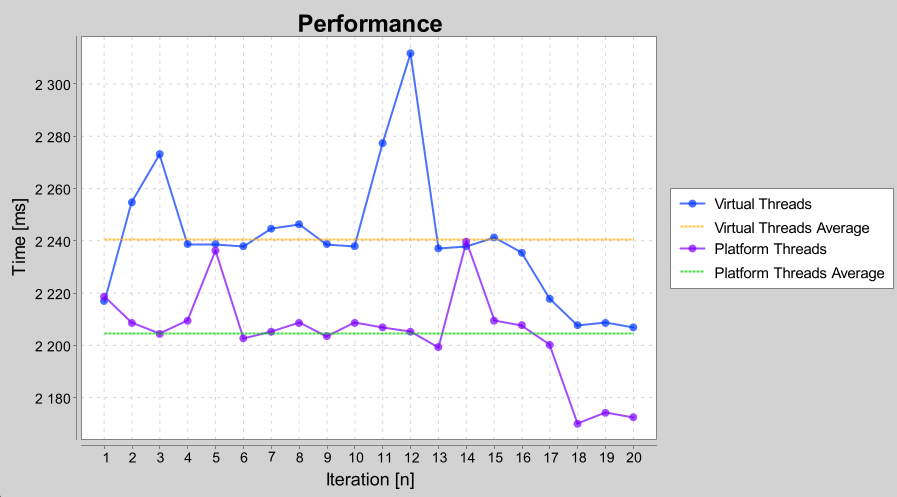
\includegraphics[width=1.0\textwidth]{Performance.png}
        \caption{Laufzeitmessungen bei Threads unter hoher Auslastung}
        \label{fig:Performance}
    \end{figure}

    Die Graphen in Abbildung \ref{fig:Performance} stellen die Ergebnisse dar. Auf der x-Achse sind die einzelnen Messiterationen abgebildet. Die y-Achse ordnet den einzelnen Messiterationen die gemessene
    Ausführungsdauer zu.
    Das arithmetische Mittel der Ausführungsdauer der \Glspl{vt} beträgt 2240,6391 Millisekunden (ms). 
    \Glspl{pt} benötigten dafür durchschnittlich 2204,6939 ms. Somit beträgt der mittlere Geschwindigkeitsunterschied 1,6 \% zugunsten der \Glspl{pt}.
    Das Ergebnis ist damit begründbar, dass in diesem Fall die von den Entwicklern genannten Verbesserungen der \Glspl{vt} keine Vorteile bieten. Weder die billigere
    Erstellung neuer Instanzen, da wenige Threads gestartet werden, noch die Fähigkeit bei blockierenden Aufgaben vom Carrier-Thread gelöst zu werden, da keine blockierenden Aufgaben auftreten und
    auch keine anderen \Glspl{vt} existieren, die diese Rechenzeit beanspruchen könnten. Nur dürfte ein kleiner Overhead existieren der sie im Vergleich zu \Glspl{pt} verlangsamt, da ein \gls{vt} alle seine
    Berechnungen auf einem \gls{pt} ausführt.
    Diese Unterschiede sollten in den meisten Fällen aber vernachlässigbar sein, da die Einbußen sich gering halten und sich solch reine Situationen wie dieser Benchmark in Praxis eher selten 
    ergeben.



\subsection{Laufzeitmessungen bei wartender Auslastung}                                         
\label{subsec:sleep}

    Der nächste Benchmark behandelt einen Fall, bei dem eine hohe Anzahl sehr wenig rechenintensiver Aufgaben parallel gestartet werden. Die Aufgaben selbst simulieren einen blockierenden
    Prozess wie beispielsweise das
    Warten auf die Antwort eines Servers. Die einzelnen Threads werden mittels Executor-Services erstellt. Gegenübergestellt werden ein \texttt{VirtualThreadPerTaskExecutor}, ein \texttt{CachedThreadPool}
    und ein \texttt{ThreadPerTaskExecutor} für \Glspl{pt}. Jeder Thread führt dann ein \texttt{Thread.sleep()} aus und gibt anschließend ein Ergebnis zurück. 
    \begin{program} [H]
        \caption{Laufzeitmessungen bei wartenden Auslastung}
        \label{prog:sleep}
    \begin{JavaCode}[language=Java, numbers=left]
@State(Scope.Benchmark)
public class VirtualThreadSleep {

    @Param("100000")
    public static int cnt;

    @Benchmark
    @BenchmarkMode(Mode.SampleTime)
    @OutputTimeUnit(TimeUnit.MILLISECONDS)
    public static void virtualExecutor() { 
        try (var executor = Executors.newVirtualThreadPerTaskExecutor()) {
            IntStream.range(0, cnt).forEach(i -> {
                Future<Integer> future = executor.submit(() -> {
                    Thread.sleep(Duration.ofSeconds(1)); return i;
                });
            });
        }
    }
}\end{JavaCode}
    \end{program}
    In Programm \ref{prog:sleep} ist die Implementierung für den \texttt{VirtualThreadPerTaskExecutor} zu sehen. Die Implementierungen der anderen beiden Benchmarks unterscheiden sich dabei nur beim verwendeten 
    Executor. Wichtig ist, bei dieser Laufzeitmessung anzumerken, dass die Anzahl an Aufgaben (Zeilen 4 und  5) höher ist als die Anzahl der vom Betriebssystem direkt bereitgestellten Threads.
    \begin{figure}[H]
        \centering
        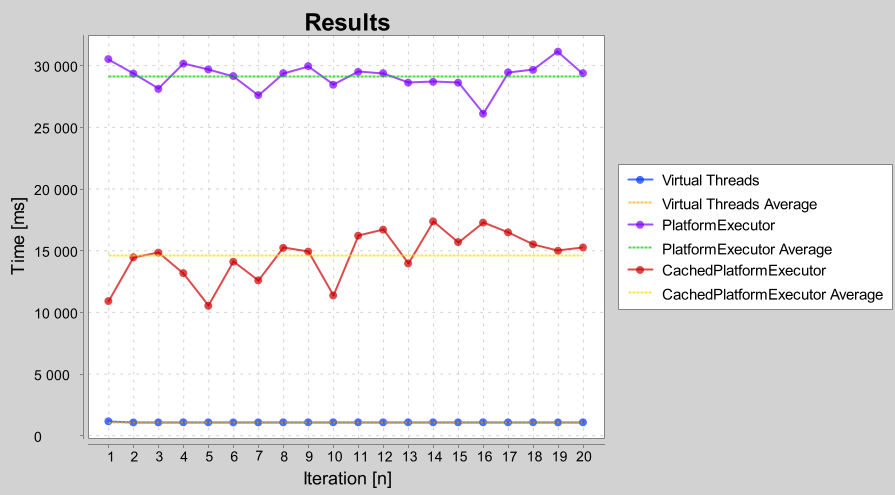
\includegraphics[width=1.0\textwidth]{sleep.png}
        \caption{Laufzeitmessungen bei wartenden Auslastung}
        \label{fig:sleep}
    \end{figure}
    Wie in der Abbildung \ref{fig:sleep} zu erkennen, fallen die Ergebnisse dieses Benchmarks sehr zugunsten der \Glspl{vt} aus. Sie benötigten im Durchschnitt  nur 1098.3845 ms. 
    Ein jeder Thread muss genau
    1000 ms warten. Daher wurden nur ca. 98 ms als Overhead benötigt um 100.000 \Glspl{vt} zu erstellen und zu verwalten. Daran, dass die Ausführungszeit einer jeden Iteration unter 2000 ms beträgt, ist
    erkennbar, dass alle Aufgaben parallel ausgeführt werden konnten.
    Der \texttt{CachedThreadPool} benötigte im Mittel 14588.2087 ms, also über das zehnfache länger als \Glspl{vt}.
    Sogar nochmal deutlich schlechter abgeschnitten hat der \texttt{ThreadPerTaskExecutor} mit einer mittleren Laufzeit von 29152.0905 ms. Somit war dieser nur etwa halb so schnell wie
    der \texttt{CachedThreadPool}. Aufgrund dieses hohen Unterschiedes ist anzunehmen, dass bei den beiden Benchmarks, die ausschließlich \Glspl{pt} nutzen, nicht alle Aufgaben parallel ausgeführt
    werden konnten. Der \texttt{CachedThreadPool} konnte die Laufzeit reduzieren, indem die Threads, die ihre Aufgaben abgeschlossen haben, wiederverwendet wurden. Somit fällt in einigen Situationen 
    die ressourcenintensive Instanziierung weg. Sollten alle Threads gleichzeitig ausführbar sein, ginge dieser Vorteil verloren. Zusätzlich wurde auch ein \texttt{ForkJoinPool} getestet. 
    Im Punkt Laufzeit schnitt dieser nur leicht besser als der \texttt{ThreadPerTaskExecutor} ab. Es ist auch anzumerken, dass 
    im Gegensatz zu allen anderen getesteten Thread-Pools beim \texttt{ForkJoinPool} nicht mehr mit dem Gerät interagiert werden konnte. Beim Versuch, im Hintergrund andere Prozesse auszuführen, kamen diese zum 
    Stillstand. 

\subsection{Laufzeitmessungen bei Abhängigkeiten zwischen Threads}
\label{subsec:LaufzeitmessungenbeiAbhängigkeitenzwischenThreads}

    Solch reine Anwendungsfälle, wie in den ersten beiden Benchmarks behandelt wurden, kommen in der Praxis natürlich nicht vor. Viel häufiger treten Mischfälle auf, in denen zwar teils rechenintensive Anweisungen
    ausgeführt werden,
    aber zusätzlich noch externe Abhängigkeiten eine Blockierung des Prozesses bewirken. Aus diesem Grund wird für einen weiteren Laufzeittest ein Produzenten-Konsumenten Modell herangezogen.
    Dabei platzieren eine Menge an Produzenten, die jeweils als ein eigener Thread implementiert sind, Objekte in eine \texttt{ArrayBlockingQueue} mit einer definierten maximalen Kapazität.
    Die Konsumenten entnehmen die Objekte wiederum aus der Warteschlange. Die \texttt{ArrayBlockingQueue} ist Thread-sicher implementiert und verhindert gleichzeitige Zugriffe. Außerdem werden 
    die Produzenten blockiert, sollte die maximale Kapazität erreicht werden. Dasselbe gilt für die Konsumenten, falls die Warteschlange leer sein sollte. 
    Damit auch rechenintensive Operationen durchgeführt werden, rufen alle Konsumenten und Produzenten beim Ausführen ihrer Arbeitsschritte die Methode \texttt{executeNonsense}, ersichtlich
    in Programm \ref{prog:executeNonsense} auf.

    \begin{figure}[H]
        \centering
        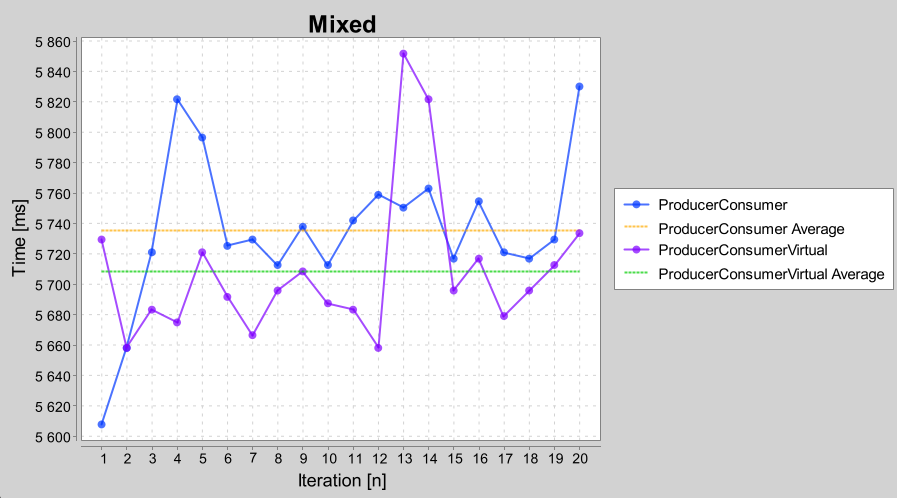
\includegraphics[width=1.0\textwidth]{mixed.png}
        \caption{Laufzeitmessungen bei Abhängigkeiten zwischen Threads}
        \label{fig:mixed}
    \end{figure}

    Die Abbildung \ref{fig:mixed} zeigt deutlich, dass der Unterschied zwischen den beiden Herangehensweisen eher gering ausfällt. Die Version mit den \Glspl{pt} benötigte im Durchschnitt 5735,2912 ms. 
    Die \Glspl{vt} waren in diesem Fall mit einer mittleren Ausführungsdauer von 5708,2711 ms um 1,5 \% schneller. Dies ist darauf zurückzuführen, dass die einzelnen Threads aufwändige Berechnungen 
    durchführen mussten bevor sie ein neues Element produzieren oder konsumieren konnten. Wären sehr viel mehr Threads dabei eingesetzt worden, die keine zusätzlichen Berechnungen durchführen müssten, wäre 
    dieser Benchmark mehr zugunsten der \Glspl{vt} ausgefallen.
    
\section{Messungen bei ScopedValues in verschiedenen Szenarien}
\label{sec:MessungenbeiScopedValuesinverschiedenenSzenarien}

    Da laut den Entwicklern und Entwicklerinnen von Projekt Loom die Klasse \texttt{ThreadLocal} in Kombination mit \Glspl{vt} zu Problemen beim Ressourcenbedarf führen kann, 
    wurden einige Messungen durchgeführt, die den Unterschied zwischen \texttt{ThreadLocal} und \texttt{Scoped\-Value} ermitteln sollen. Getestet wurden dabei verschiedene Szenarien
    unter der exklusiven Verwendung von \Glspl{vt}. 
    Als besonders schwierig stellte sich dabei die Ermittlung des Speicherverbrauchs dar, da die meisten Werkzeuge wie \texttt{MemoryMXBean} oder \texttt{org.github.jamm} die Neuerungen von 
    Projekt Loom noch nicht unterstützen.

\subsection{Laufzeit bei einzelnen Abfragen}
\label{sec:LaufzeitbeieinzelnenAbfragen}
    
    Ziel dieses Benchmarks ist es, die Klassen \texttt{ThreadLocal} und \texttt{ScopedValue} hinsichtlich Laufzeit bei einer Wertzuweisung und einer einzelnen Wertabfrage gegenüberzustellen.
    Dieses Szenario ist deswegen interessant, da bei der Verwendung von \texttt{ScopedValue} Caching erst bei wiederholten Abfragen zum Einsatz kommt. Bei der Nutzung von Thread-lokalen Variablen
    liegt der Wert immer direkt am Thread-Objekt selbst. 

    \begin{program} [H]
        \caption{Laufzeit bei einzelnen Abfragen}
        \label{prog:SingleQuery}
    \begin{JavaCode}[language=Java, numbers=left]
@BenchmarkMode(Mode.SampleTime)
@State(Scope.Thread)
@OutputTimeUnit(TimeUnit.SECONDS)
public class ScopedValueBenchmarkSingleQuery {
    private static final ScopedValue<String> sv = ScopedValue.newInstance();

    @Param({"100000"})
    private int numThreads;

    @Benchmark
    public void testScopedValue() throws Exception {
        try(var executor = Executors.newVirtualThreadPerTaskExecutor()) {
            for (int i = 0; i < numThreads; i++) {
                executor.execute(() -> ScopedValue.where(sv, "ScopedValue")
                .run(() -> { String value = sv.get(); }));
            }
        }
    }
}\end{JavaCode}
    \end{program}

    Wie in Programm \ref{prog:SingleQuery} zu sehen ist, wird in dem Beispiel eine einzelne Instanz der Klasse \texttt{ScopedValue} verwendet. Im Benchmark selbst wird ein Executor-Service benutzt, um eine
    in Zeile 7 definierte Anzahl an Threads zu starten, um den Einfluss externer Faktoren zu verringern. In jedem Thread geschieht eine Bereichs- und Wertzuweisung der Variable.
    Anschließend wird der Wert der Variable wieder abgefragt. Die Testklasse für \texttt{ThreadLocal} unterscheidet sich nur darin, dass ein \texttt{TreadLocal}-Objekt benutzt wird, um den Wert
    abzuspeichern.

    \begin{figure}[H]
        \centering
        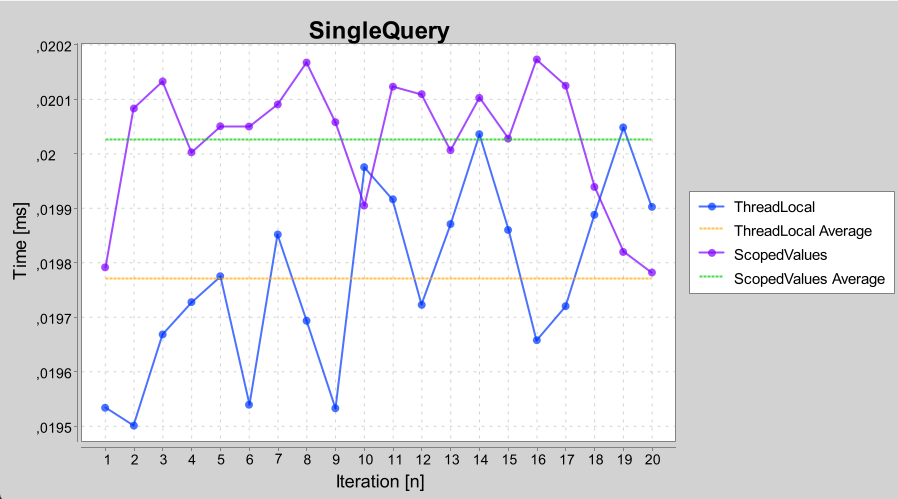
\includegraphics[width=1.0\textwidth]{SingleQuery.png}
        \caption{Laufzeitmessungen bei einzelnen Abfragen}
        \label{fig:SingleQuery}
    \end{figure}

    In \ref{fig:SingleQuery} ist zu erkennen, dass der Unterschied zwischen den beiden Technologien in diesem Anwendungsfall gering ausfällt. Mit einer durchschnittlichen Ausführungsdauer von
    0,01977 ms war die Implementierung mit \texttt{ThreadLocal} um etwa 1,2 \% schneller als die Alternative. Die Implementierung mit \texttt{ScopedValue} benötigte im Mittel 0,02002 ms.
    Diese Messungen beinhalten auch die Zeit, die benötigt wurde, um die Objekte selbst zu erstellen und zu die Wertzuweisungen durchzuführen. Sollte dieser Vorgang bei einer der beiden Technologien 
    langsamer als bei der anderen erfolgen, könnte dies dazu führen, dass die Abfrage dafür um einiges schneller erfolgt als vermutet. Eine Berücksichtigung dieser Eigenschaft wäre für den praktischen
    Gebrauch wenig zielführend, da eine einzelne Wertabfrage ohne Wertzuweisung nicht durchführbar ist. 

\subsection{Laufzeit bei wiederholten Abfragen}
\label{sec:LaufzeitbeiwiederholtenAbfragen}

    Wie in Kapitel \ref{subsec:UnterschiedeScopedValuesundThreadLocal} bereits erwähnt, werden bereichsgebundene Variablen beim ersten Aufruf der Methode \texttt{get()} ebenfalls im Thread-Objekt 
    zwischengespeichert. Wenn dieser Zwischenspeicher nicht überfüllt wird, sollte dies zu einem Zuwachs der Zugriffsgeschwindigkeit führen. In diesem Testszenario wird dies überprüft.
    Die Testklasse selbst gleicht jener aus Programm \ref{prog:SingleQuery}. Der Unterschied liegt lediglich darin, dass in jedem Thread mehrere Zugriffe auf den Wert der Variable erfolgen. Eine 
    Wertzuweisung erfolgt hingegen ebenfalls wieder nur einmal zu Beginn.


    \begin{figure}[H]
        \centering
        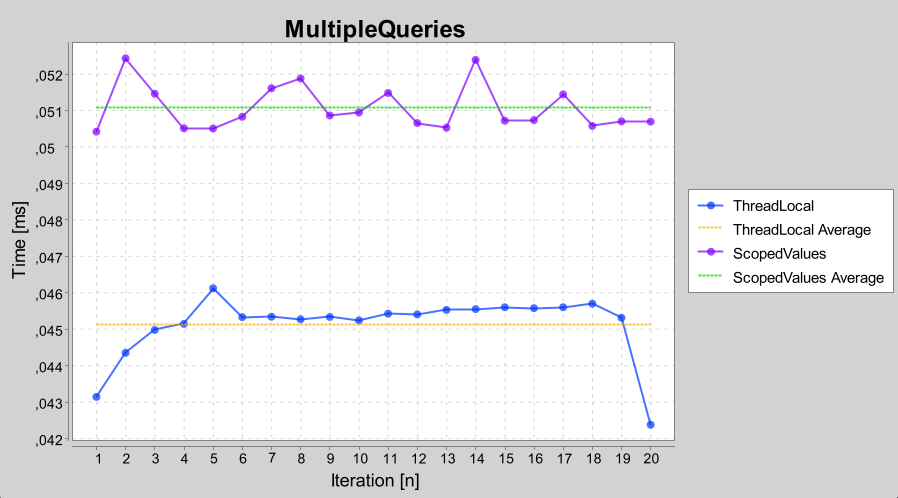
\includegraphics[width=1.0\textwidth]{MultQuery.png}
        \caption{Laufzeitmessungen bei wiederholten Abfragen}
        \label{fig:MultQuery}
    \end{figure}

    Der Fakt, dass bei wiederholten Wertabfragen von bereichsgebundenen Variablen der Wert am Thread selbst zwischengespeichert werden sollte, lässt vermuten, dass der Unterschied zu Threadlokal 
    sehr gering ausfallen sollte. Dies ist in diesem Szenario, wie in Abbildung \ref{fig:MultQuery} zu sehen ist, nicht der Fall. Der Test für die Klasse \texttt{ThreadLocal} benötigte
    durchschnittlich 0,045122 ms. Der Test für \texttt{ScopedValue} benötigte mit 0,051074 ms etwa 13 \% mehr Zeit. Berücksichtigt man auch die Ergebnisse aus Kapitel \ref{sec:LaufzeitbeieinzelnenAbfragen}
    ist anzunehmen, dass bei der Klasse \texttt{ScopedValue} die Instanziierung und Wertbindung schneller erfolgt als bei \texttt{ThreadLocal}. Dafür benötigt die Wertabfrage mehr Zeit, auch bei einer 
    Zwischenspeicherung des Wertes direkt am Thread-Objekt.

\subsection{Laufzeit bei Thread-übergreifender Vererbung der Variablen}
\label{sec:LaufzeitbeiVererbung}

    Das Verhalten von \texttt{InheritableThreadLocal} wurde von den Entwicklern der \Glspl{vt} in Kombination mit einer hohen Anzahl an kurzlebigen Threads als potentiell problematisch 
    dargestellt. Diese Laufzeitmessung stellt daher den Vererbungsvorgang von \texttt{InheritableTreadLocal} und \texttt{ScopedValue} gegenüber.

    \begin{program} [H]
        \caption{Laufzeit bei Vererbung}
        \label{prog:Inheritance}
    \begin{JavaCode}[language=Java, numbers=left]
@BenchmarkMode(Mode.SampleTime)
@State(Scope.Thread)
@OutputTimeUnit(TimeUnit.SECONDS)
public class ScopedValuesInheritanceBenchmark {
    private static final ScopedValue<String> sv = ScopedValue.newInstance();

    @Param({"100000"})
    private int cnt;

    @Benchmark
    public void test(){
        ScopedValue.where(sv, "parent").run(() -> {
            try (var scope = new StructuredTaskScope<Void>()) {
                for (int i = 0; i < cnt; i++) 
                    scope.fork(() -> {int j = 0; return null; });
                scope.join();
            } catch (InterruptedException e) {
                throw new RuntimeException(e);
            }
        });
    }
}\end{JavaCode}
    \end{program}
    Da die threadübergreifende Vererbung eines bereichsgebundenen Wertes nur stattfindet, wenn der neue Thread durch die \texttt{fork}-Methode eines \gls{sts} erstellt wurde, wird eine Instanz 
    der Basisklasse \texttt{StructuredTaskScope} verwendet. Im neuen Thread selbst wird nicht mehr auf
    den Wert zugegriffen, da dieser Vorgang in den beiden Situationen unterschiedliche Performanz aufweisen kann. Stattdessen wird eine einfache Instruktion mit einer konstanten Ausführungsdauer
    durchgeführt. Ein \gls{sts} erwartet bei jeder Teilaufgabe einen retournierten Wert, daher ist das zweite Statement in Zeile 15 nötig. Um eine \texttt{StructureViolationException} zu vermeiden,
    müssen sich sowohl der gesamte \gls{sts}, als auch die Instanziierung und der \texttt{join()}-Aufruf im Gültigkeitsbereich einer Wertbindung des \texttt{ScopedValue} befinden.
    Die Vergleichsmessung
    nutzt eine Instanz der Klasse \texttt{InheritableTreadLocal}. In Zeile 12 wird der Wert mittels der \texttt{set()}-Methode festgelegt.

    \begin{figure}[H]
        \centering
        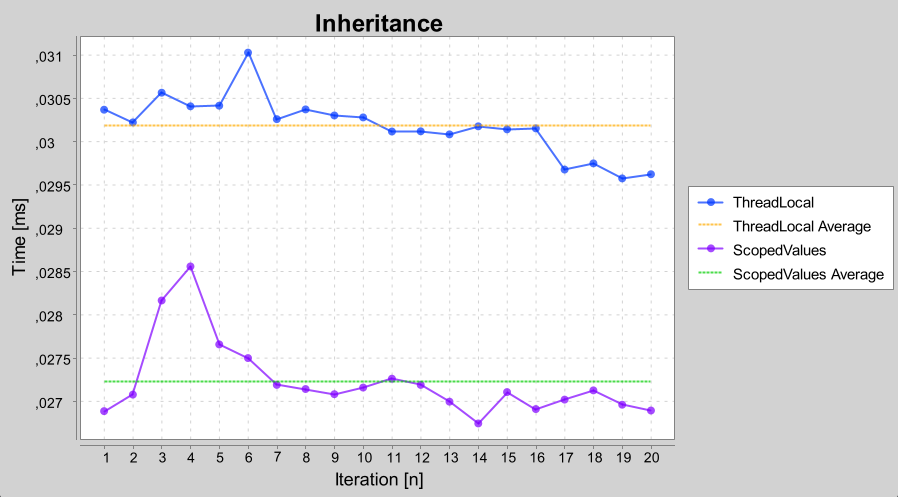
\includegraphics[width=1.0\textwidth]{Inheritance.png}
        \caption{Laufzeitmessungen bei Vererbung}
        \label{fig:inheritance}
    \end{figure}

    Der Test für bereichsgebundene Werte benötigte in diesem Szenario im Durchschnitt 0.02723 ms. Die Ausführung der Version mit \texttt{ThreadLocal} war mit 0.03018 ms um etwa 10 \% langsamer. 
    Bei Threads mit einer sehr kurzen Lebensdauer könnte dieser Geschwindigkeitsunterschied bedenklich sein, wobei vorher abgewogen werden sollte, ob eine Vererbung der Werte überhaupt 
    benötigt wird. Bereichsgebundene Variablen können zwar beschleunigen, doch die Auswahl sollte anhand der benötigten Eigenschaften erfolgen, wie beispielsweise der Veränderbarkeit.

\subsection{Speicherbedarf bei einer hohen Anzahl an Threads}
\label{sec:Speicherbedarf}

    Interessant ist ebenfalls die Gegenüberstellung der beiden Technologien im Bezug auf ihren Speicherbedarf. Dazu wird ein \texttt{byte}-Feld mit 1.048.576 Einträgen erstellt und als Wert für einen
    \texttt{ScopedValue} benutzt. Dieser Wert wird dann auf 1000 neue \Glspl{vt} vererbt. Dazu kommt ein \gls{sts} zum Einsatz. Direkt vor und nach dem \gls{sts} wird mittels 
    \texttt{MemoryMXBean} der von der \gls{jvm} verwendete Speicher ermittelt. Nach kurzem Warten und einem Aufruf von \texttt{System.gc()}, um den Garbage-Collector zu aktivieren, wird 
    dieser Vorgang für \texttt{InheritableThreadLocal} wiederholt. Nach 5 Messiterationen konnte festgestellt werden, dass \texttt{InheritableThreadLocal} einen 137-fachen Speicherbedarf 
    vorweist, obwohl in jedem Thread ein Zugriff auf den Wert durchgeführt wurde, damit das Caching bei \texttt{ScopedValue} durchgeführt werden könnte. Dieses Verhalten weist darauf hin, dass
    das Zwischenspeichern des Wertes am Thread-Objekt bei \texttt{ScopedValue} in diesem Fall nur begrenzt oder gar nicht durchgeführt wurde. Auch wenn die Methode zur Ermittlung des Speicherbedarfs 
    nicht unbedingt präzise ist, stellt sich das Ergebnis als so aussagekräftig heraus, um einen Schluss ziehen zu können. Sollten viele Threads benötigt werden und der bereitgestellte Wert 
    nicht in jedem Thread benötigt werden, stellt sich \texttt{ScopedValue} als wesentlich speichersparender heraus. Der Quelltext ist im Anhang in Programm \ref{prog:Speicherverbrauch} zu finden.
